\documentclass[11pt,a4paper]{article}

% ---------- pacchetti ----------
\usepackage[T1]{fontenc}
\usepackage[utf8]{inputenc}
\usepackage[a4paper,margin=2.4cm]{geometry}
\usepackage{graphicx}
\usepackage{booktabs}
\usepackage{tabularx}
\usepackage{xltabular}
\usepackage{amsmath}
\usepackage{amssymb}
\usepackage{xcolor}
\usepackage{enumitem}
\usepackage{fancyhdr}
\usepackage{tcolorbox}
\usepackage{caption}
\usepackage[hidelinks]{hyperref}

\tcbuselibrary{skins,breakable}
\graphicspath{{outputs/}{./}}

% ---------- colori ----------
\definecolor{perche}{RGB}{0,102,153}
\definecolor{perchebg}{RGB}{232,244,250}
\definecolor{terminebg}{RGB}{245,240,230}
\definecolor{darkrule}{RGB}{60,60,60}

% ---------- box "PERCHE'" (motivo dello step) ----------
\newtcolorbox{perchebox}{
  enhanced, breakable, colback=perchebg, colframe=perche,
  boxrule=0.4pt, left=8pt, right=8pt, top=6pt, bottom=6pt,
  fonttitle=\bfseries, title={Perch\'e questo step}}

% ---------- box "TERMINE" (spiegazione acronimo/concetto) ----------
\newtcolorbox{terminebox}[1]{
  enhanced, breakable, colback=terminebg, colframe=darkrule,
  boxrule=0.4pt, left=8pt, right=8pt, top=6pt, bottom=6pt,
  fonttitle=\bfseries, title={#1}}

% ---------- intestazione ----------
\pagestyle{fancy}
\fancyhf{}
\rhead{\small Face Anti-Spoofing --- guida personale}
\lhead{\small Biometric Systems}
\cfoot{\thepage}
\renewcommand{\headrulewidth}{0.3pt}

\setlist{itemsep=2pt, topsep=3pt}

% comando rapido per acronimo
\newcommand{\acr}[1]{\textbf{#1}}
% virgolette
\newcommand{\say}[1]{``#1''}

\title{\vspace{-1.5cm}\textbf{Face Anti-Spoofing}\\[4pt]
\large Come funziona tutto il progetto --- guida personale per capirlo}
\author{Progetto Biometric Systems}
\date{\today}

\begin{document}
\maketitle
\thispagestyle{fancy}

\begin{tcolorbox}[colback=perchebg,colframe=perche,boxrule=0.4pt]
\textbf{A cosa serve questo documento.} Non \`e la relazione ufficiale da consegnare.
\`E una spiegazione, passo per passo, di \emph{tutto} quello che abbiamo costruito: cosa fa
ogni pezzo, \textbf{perch\'e} l'abbiamo fatto, e cosa significano i termini tecnici. L'obiettivo
\`e che tu capisca la \say{baracca} a fondo, abbastanza da spiegarla a voce.
\end{tcolorbox}

\tableofcontents
\vspace{0.4cm}
\hrule

% =====================================================================
\section{In una frase: cosa fa il sistema}
% =====================================================================
Costruiamo un sistema che, data l'immagine di un volto, decide se \`e una \textbf{persona vera
davanti alla camera} (\emph{live}) oppure un \textbf{attacco} (\emph{spoof}): una foto stampata,
una foto mostrata su uno schermo, un video in replay. Questo problema si chiama
\textbf{Face Anti-Spoofing} (o \emph{Presentation Attack Detection}).

\begin{terminebox}{Perch\'e serve --- il problema}
Un normale sistema di riconoscimento facciale (es. lo sblocco del telefono) confronta due volti.
Ma se mostro alla camera una \emph{foto} del proprietario, il sistema potrebbe sbloccarsi lo
stesso: \`e stato \say{ingannato}. L'anti-spoofing \`e il modulo che sta \emph{prima} del
riconoscimento e blocca questi tentativi. \`E un classificatore binario: \textbf{live vs spoof}.
\end{terminebox}

Abbiamo affrontato il problema in due modi diversi e poi li abbiamo combinati:
\begin{enumerate}
  \item un metodo \textbf{classico} (estrazione manuale di feature di texture + classificatore \acr{SVM});
  \item un metodo \textbf{deep learning} (una rete neurale \acr{CNN} che impara le feature da sola);
  \item la \textbf{fusione} dei due.
\end{enumerate}
Abbiamo poi misurato quanto il sistema generalizza su un \textbf{secondo dataset mai visto}
(la parte pi\`u interessante) e costruito una \textbf{demo} che funziona con la webcam. Infine
(Fase 11) abbiamo aggiunto lo stadio di \textbf{riconoscimento del volto}: cos\`i il progetto non
fa solo anti-spoofing ma diventa un \textbf{sistema biometrico completo} (anti-spoof + \say{chi sei?}).

% =====================================================================
\section{Glossario: tutti gli acronimi}
% =====================================================================
Tienilo a portata di mano: ogni termine ricompare nelle sezioni successive.

\begin{description}[style=nextline,leftmargin=1.2cm]
  \item[PAD / FAS] \textit{Presentation Attack Detection} / \textit{Face Anti-Spoofing}: il
    nostro task. Distinguere un volto reale (\emph{bonafide}) da un attacco di presentazione.
  \item[live / spoof] Le due classi. \textbf{live} = persona vera (label 0).
    \textbf{spoof} = attacco: foto, schermo, stampa (label 1).
  \item[bonafide] Sinonimo \say{ufficiale} (standard ISO) di \emph{live}: presentazione genuina.
  \item[CNN] \textit{Convolutional Neural Network}: rete neurale per immagini. Impara da sola
    quali pattern guardare, a differenza del metodo classico dove le feature le scegliamo noi.
  \item[ResNet-18] L'architettura di CNN che usiamo (18 livelli, con \say{collegamenti residui}).
    \`E pre-addestrata su ImageNet.
  \item[ImageNet] Enorme dataset di immagini generiche (1000 categorie). Le reti pre-addestrate
    su ImageNet partono gi\`a sapendo riconoscere bordi, texture, forme: ottimo punto di partenza.
  \item[SVM] \textit{Support Vector Machine}: classificatore classico. Cerca il confine che
    separa meglio le due classi. Lo usiamo con kernel \acr{RBF}.
  \item[RBF] \textit{Radial Basis Function}: il \say{kernel} che permette all'SVM di tracciare
    confini curvi (non solo rette) tra le classi.
  \item[LBP] \textit{Local Binary Pattern}: descrittore di \textbf{texture}. Per ogni pixel
    guarda i vicini e produce un codice; l'istogramma di questi codici descrive la \say{grana}
    dell'immagine. Cuore del metodo classico.
  \item[YCbCr / HSV] Spazi colore alternativi all'RGB. Separano luminanza e crominanza:
    gli artefatti dello spoof si vedono meglio nei canali di colore.
  \item[EER] \textit{Equal Error Rate}: la metrica principale. \`E il valore in cui i due tipi
    di errore (\acr{FAR} e \acr{FRR}) si eguagliano. \textbf{Pi\`u basso = meglio.}
  \item[FAR] \textit{False Acceptance Rate}: frazione di \textbf{spoof accettati come live}
    (l'errore \say{pericoloso}: un attacco passa).
  \item[FRR] \textit{False Rejection Rate}: frazione di \textbf{live rifiutati come spoof}
    (l'errore \say{fastidioso}: un utente vero viene bloccato).
  \item[ROC] \textit{Receiver Operating Characteristic}: curva che mostra il compromesso tra
    veri positivi e falsi positivi al variare della soglia.
  \item[AUC] \textit{Area Under the Curve} (della ROC): un numero in $[0,1]$ che riassume la
    bont\`a del classificatore. \textbf{1 = perfetto}, 0,5 = a caso.
  \item[DET] \textit{Detection Error Tradeoff}: curva FAR vs FRR; un altro modo standard di
    visualizzare gli errori in biometria.
  \item[APCER / BPCER / ACER] Metriche dello standard \textbf{ISO/IEC 30107-3}.
    APCER = errore sugli attacchi (spoof presi per veri), BPCER = errore sui bonafide
    (veri presi per attacco), ACER = media dei due.
  \item[HTER] \textit{Half Total Error Rate} $=(\text{FAR}+\text{FRR})/2$. Usato nel
    cross-dataset, quando la soglia \`e \textbf{fissata in anticipo} e non ri-tarata.
  \item[AMP] \textit{Automatic Mixed Precision}: durante il training usa numeri a 16 bit dove
    possibile $\Rightarrow$ pi\`u veloce e meno memoria GPU, senza perdere qualit\`a.
  \item[GPU / VRAM] La scheda grafica (NVIDIA RTX 2060 SUPER, 8 GB di memoria) su cui giriamo
    il training della CNN.
  \item[OOM] \textit{Out Of Memory}: errore di memoria esaurita. Lo abbiamo evitato (vedi Fase 2).
  \item[data augmentation] Trasformazioni casuali applicate alle immagini in training (ritaglio,
    flip, blur, compressione JPEG\dots) per rendere il modello pi\`u robusto.
\end{description}

% =====================================================================
\section{La pipeline a colpo d'occhio}
% =====================================================================
Il progetto \`e diviso in fasi, ognuna con una \say{verifica} (gate) prima di passare alla
successiva. Schema:

\begin{center}
\small
\begin{tabular}{@{}rl@{}}
\toprule
\textbf{Fase} & \textbf{Cosa produce} \\
\midrule
1. Setup        & ambiente Python + GPU pronti \\
2. Dataset      & 146k immagini live/spoof su disco + indici CSV \\
3. Preprocessing & transforms e data augmentation \\
4. Baseline     & SVM su feature LBP $\rightarrow$ \emph{il riferimento da battere} \\
5. CNN          & ResNet-18 fine-tuned $\rightarrow$ il modello forte \\
6. Valutazione  & metriche + grafici di confronto \\
7. Cross-dataset & test su un dataset mai visto (il domain gap) \\
8. Fusione      & combinazione SVM + CNN a livello di score \\
9. Demo         & inferenza su immagine e webcam in tempo reale \\
11. Recognition & embedding + identificazione open-set $\rightarrow$ \emph{sistema completo} \\
\bottomrule
\end{tabular}
\end{center}

\begin{perchebox}
Lavorare a fasi con un gate dopo ognuna evita di accorgersi alla fine che qualcosa, a monte,
era sbagliato. Ogni fase produce un artefatto verificabile (un numero, un grafico, un file)
prima di costruirci sopra la successiva. \`E lo stesso principio dei test in ingegneria del software.
\end{perchebox}

% =====================================================================
\section{Fase 1 --- Setup dell'ambiente}
% =====================================================================
\textbf{Cosa.} Abbiamo creato un ambiente Python isolato (\texttt{.venv}) e installato PyTorch
(con supporto \acr{GPU} CUDA), \texttt{timm} (le architetture pronte), OpenCV, scikit-learn,
scikit-image. Verificato che la GPU sia vista da PyTorch.

\begin{perchebox}
Una \textbf{virtualenv} tiene le librerie del progetto separate dal sistema: versioni
riproducibili, niente conflitti. La verifica della GPU \`e fondamentale perch\'e addestrare una
CNN su CPU sarebbe lentissimo: sulla RTX 2060 un'epoca dura $\sim$5 minuti, su CPU sarebbe ore.
\end{perchebox}

\textit{Nota pratica:} le dipendenze sono in \texttt{requirements.txt}. PyTorch va installato a
parte dall'indice ufficiale (il pacchetto con CUDA non sta su PyPI).

% =====================================================================
\section{Fase 2 --- Il dataset}
% =====================================================================
\textbf{Cosa.} Abbiamo usato \textbf{CelebA-Spoof}, uno dei pi\`u grandi dataset pubblici di
anti-spoofing, nella versione \emph{cropped} (volti gi\`a ritagliati) presa da Hugging Face.
Scaricato un sottoinsieme ($\sim$12 GB di file \texttt{parquet}), poi \textbf{estratto in PNG su
disco} con un indice \texttt{.csv} (colonne \texttt{filepath, label}).

\begin{center}
\small
\begin{tabular}{@{}lrrr@{}}
\toprule
\textbf{Split} & \textbf{Immagini} & \textbf{Live} & \textbf{Spoof} \\
\midrule
TRAIN              & 79.183 & 33,2\% & 66,8\% \\
\quad$\rightarrow$ train (fit)        & 67.306 & 33,0\% & 67,0\% \\
\quad$\rightarrow$ val (early stop)   & 11.877 & 34,1\% & 65,9\% \\
TEST (disgiunto)   & 66.787 & 29,7\% & 70,3\% \\
\bottomrule
\end{tabular}
\end{center}

\begin{perchebox}
\textbf{Perch\'e un dataset grande e pubblico:} servono decine di migliaia di esempi per
addestrare una CNN senza che impari \say{a memoria}; ed essendo pubblico i risultati sono
confrontabili con la letteratura.\\[4pt]
\textbf{Perch\'e estrarre i PNG su disco:} caricare tutti i parquet (con le immagini dentro) in
RAM la saturava $\rightarrow$ errore \acr{OOM}. Scrivendo i file su disco una volta sola, il
training legge ogni immagine \say{on-the-fly} con poca memoria. \\[4pt]
\textbf{Perch\'e tre split (train/val/test):}
\emph{train} = su cui il modello impara;
\emph{val} = per decidere quando fermarsi e tarare la soglia (\textbf{non} per imparare);
\emph{test} = il \say{compito d'esame}, visto solo alla fine per dare il voto onesto.
\end{perchebox}

\begin{terminebox}{Concetto chiave: il \say{data leakage} e perch\'e il test \`e separato}
Se il modello vedesse in fase di test gli stessi dati (o lo stesso soggetto) su cui si \`e
allenato, otterrebbe un voto gonfiato e bugiardo. Qui il \textbf{test viene dallo split ufficiale
disgiunto} di CelebA-Spoof, quindi soggetti diversi: la valutazione finale \`e pulita. Il
\emph{val}, ricavato dal train, pu\`o condividere soggetti col train, ma va bene perch\'e serve
solo a fermare il training al momento giusto, non a dare il voto.
\end{terminebox}

\textbf{Nota sullo sbilanciamento.} Ci sono circa il doppio di spoof rispetto a live ($\sim$2:1).
Se non facessimo nulla, il modello sarebbe \say{pigro} e tenderebbe a dire sempre \say{spoof}.
Lo gestiamo nelle fasi successive con i \emph{class weights} / sottocampionamento bilanciato.

% =====================================================================
\section{Fase 3 --- Preprocessing e data augmentation}
% =====================================================================
\textbf{Cosa.} Poich\'e i volti sono gi\`a ritagliati, il preprocessing si riduce a:
ridimensionare a $224\times224$, normalizzare con le statistiche di ImageNet, e --- solo in
training --- applicare \textbf{augmentation casuale}: ritaglio, flip orizzontale, variazioni di
colore/luminosit\`a, sfocatura, \textbf{ricompressione JPEG casuale}, cancellazione di una zona
(random erasing).

\begin{figure}[h]
\centering
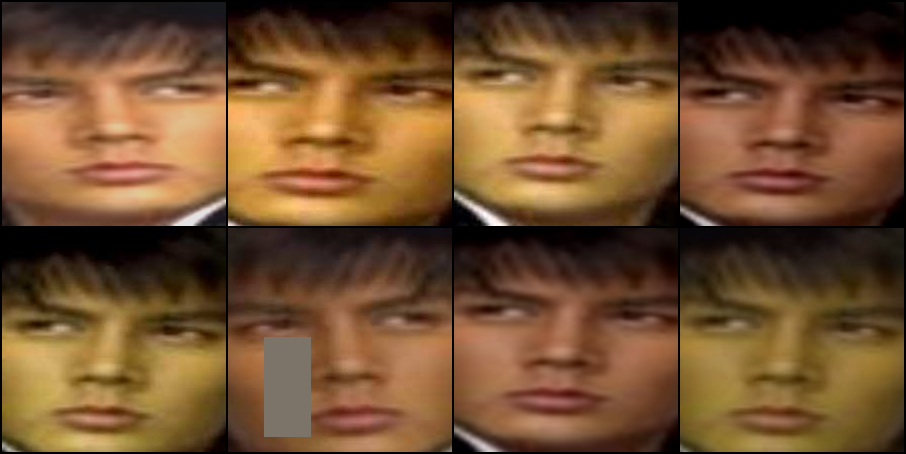
\includegraphics[width=0.9\textwidth]{aug_preview.png}
\caption{Esempi di immagini dopo l'augmentation: ogni copia \`e leggermente diversa.}
\end{figure}

\begin{perchebox}
\textbf{Perch\'e normalizzare con le statistiche di ImageNet:} la CNN \`e pre-addestrata su
ImageNet, quindi si aspetta input con quella scala di colori; rispettarla rende il
fine-tuning pi\`u stabile.\\[4pt]
\textbf{Perch\'e l'augmentation (e proprio queste trasformazioni):} mostrando al modello molte
varianti della stessa immagine gli impediamo di imparare dettagli irrilevanti (\say{overfitting})
e lo rendiamo \textbf{robusto}. In particolare blur e \textbf{JPEG casuale} imitano gli artefatti
di stampa e di replay: \`e l'augmentation che aiuter\`a di pi\`u nel cross-dataset (Fase 7).
\end{perchebox}

% =====================================================================
\section{Fase 4 --- Baseline classica: LBP + SVM}
% =====================================================================
\textbf{Cosa.} Prima di tirare fuori il deep learning costruiamo un \textbf{metodo di riferimento}
semplice e classico, basato sull'articolo di Boulkenafet et al.\ (2015):
\begin{enumerate}
  \item per ogni immagine calcoliamo istogrammi \acr{LBP} (texture) su due spazi colore
        (\acr{YCbCr} e \acr{HSV}), su pi\`u scale, per ogni canale $\rightarrow$ un vettore di
        \textbf{168 numeri} che descrive la \say{grana} dell'immagine;
  \item addestriamo un \acr{SVM} con kernel \acr{RBF} a separare live da spoof su questi vettori.
\end{enumerate}

\begin{terminebox}{Perch\'e la texture distingue live da spoof}
Una foto reale e la \emph{foto di una foto} hanno micro-texture diverse: lo schermo aggiunge
pattern di pixel (effetto moir\'e), la stampa aggiunge grana e riflessi, la ricompressione
aggiunge artefatti. L'\acr{LBP} cattura proprio questi pattern locali, e sono pi\`u evidenti nei
\textbf{canali di colore} (per questo YCbCr/HSV e non solo RGB).
\end{terminebox}

\begin{perchebox}
\textbf{Perch\'e fare una baseline prima della CNN:} ti d\`a un \textbf{metro di paragone} onesto.
Senza, non sapresti se l'EER della CNN \`e \say{buono}. La baseline risponde alla domanda
\say{quanto \`e difficile questo problema con metodi semplici?}. \\[4pt]
\textbf{Perch\'e un sottocampione bilanciato per l'SVM:} l'SVM RBF non scala a decine di migliaia
di esempi (diventa lentissimo) ed \`e sensibile allo sbilanciamento; addestriamo su 12.000
immagini bilanciate. La \textbf{valutazione} \`e per\`o sul test completo (66.787 immagini).
\end{perchebox}

\textbf{Risultato:} \textbf{EER = 7,69\%}, AUC = 0,976. \`E il numero da battere.

% =====================================================================
\section{Fase 5 --- Il modello deep: CNN fine-tuned}
% =====================================================================
\textbf{Cosa.} Prendiamo una \textbf{ResNet-18 pre-addestrata su ImageNet}, le sostituiamo
l'ultimo strato con uno a 2 uscite (live/spoof) e la ri-addestriamo (\emph{fine-tuning}) sul
nostro dataset. Dettagli del training:
\begin{itemize}
  \item \textbf{AMP} (mixed precision) per stare negli 8 GB di VRAM ed essere veloci;
  \item \textbf{class weights} (peso maggiore alla classe meno frequente) per lo sbilanciamento 2:1;
  \item \textbf{early stopping} sull'EER di validation: ci fermiamo quando smette di migliorare;
  \item scheduler \emph{cosine} che riduce gradualmente il learning rate.
\end{itemize}
5 epoche, $\sim$24 minuti totali sulla GPU.

\begin{figure}[h]
\centering
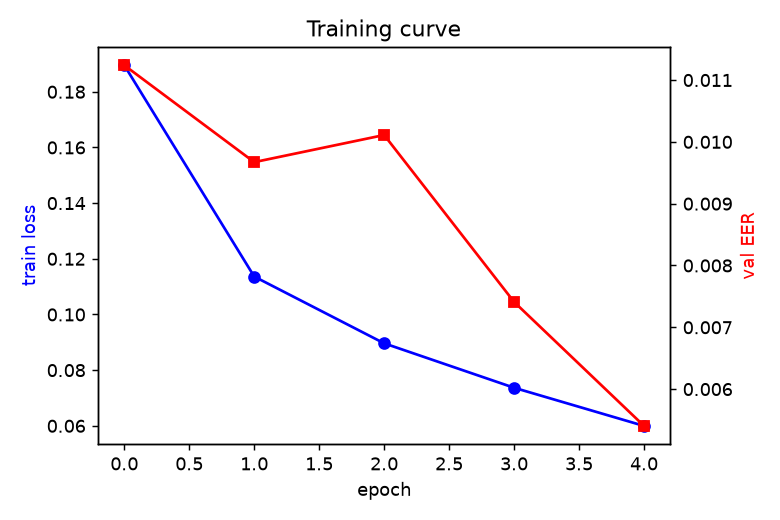
\includegraphics[width=0.62\textwidth]{train_curve.png}
\caption{Curva di training: la loss (blu) scende, l'EER di validation (rosso) scende fino a
$\sim$0,5\%. Nessun overfitting (le due curve scendono insieme).}
\end{figure}

\begin{terminebox}{Cos'\`e il \say{transfer learning} / fine-tuning}
Invece di partire da una rete \say{a caso}, partiamo da una gi\`a addestrata a riconoscere
immagini generiche (ImageNet). Sa gi\`a vedere bordi, texture, forme; noi le insegniamo solo la
nuova distinzione live/spoof. Risultato: ottimi risultati con \textbf{poco tempo e pochi dati}
rispetto ad addestrare da zero.
\end{terminebox}

\begin{perchebox}
\textbf{Perch\'e una CNN se la baseline gi\`a funziona:} la CNN \textbf{impara da sola} quali
dettagli guardare, anche quelli che noi non sapremmo descrivere a mano con l'LBP. Ci aspettiamo
(e otteniamo) un netto miglioramento.\\[4pt]
\textbf{Perch\'e early stopping sul \emph{val}:} continuare ad allenare troppo a lungo fa
\say{imparare a memoria} il train (overfitting). Fermarci quando il val smette di migliorare ci
d\`a il modello che generalizza meglio. \textbf{Perch\'e i class weights:} per non far ignorare al
modello la classe live (minoritaria).
\end{perchebox}

\textbf{Risultato:} \textbf{EER = 3,69\%}, AUC = 0,994. La CNN \textbf{dimezza l'errore} della
baseline (7,69\% $\rightarrow$ 3,69\%).

% =====================================================================
\section{Fase 6 --- Valutazione e confronto}
% =====================================================================
\textbf{Cosa.} Abbiamo un modulo unico che carica gli score salvati dei due modelli, ricalcola
tutte le metriche e disegna le curve \acr{ROC} e \acr{DET} \textbf{sovrapposte}, pi\`u una tabella
riassuntiva.

\begin{center}
\small
\begin{tabular}{@{}lrrr@{}}
\toprule
\textbf{Modello (test, 66.787 img)} & \textbf{EER} & \textbf{AUC} & \textbf{ACER} \\
\midrule
Baseline SVM (color-LBP) & 7,69\% & 0,976 & 7,69\% \\
CNN (ResNet-18)          & \textbf{3,69\%} & \textbf{0,994} & \textbf{3,69\%} \\
\bottomrule
\end{tabular}
\end{center}

\begin{figure}[h]
\centering
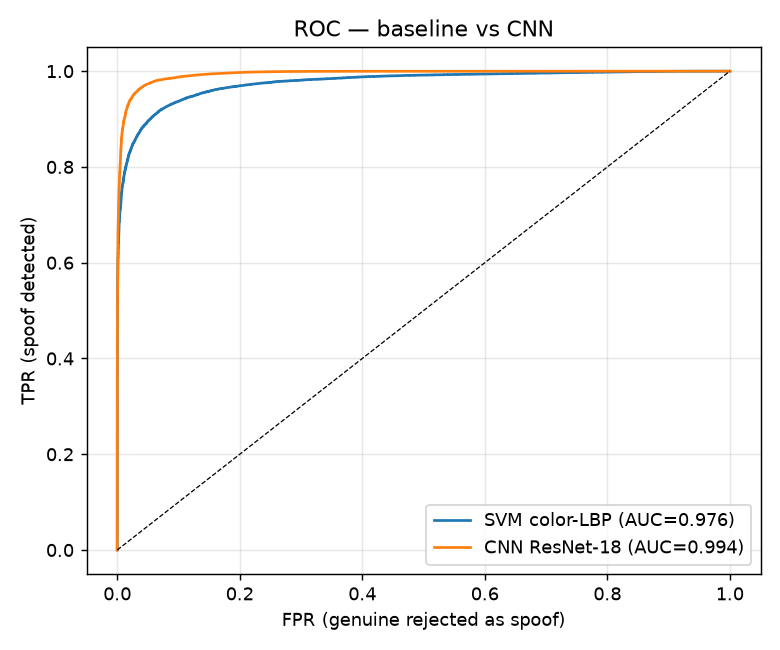
\includegraphics[width=0.6\textwidth]{roc_compare.png}
\caption{ROC a confronto: la curva della CNN \say{abbraccia} l'angolo in alto a sinistra
(meglio). Pi\`u l'area sotto la curva (AUC) si avvicina a 1, migliore \`e il modello.}
\end{figure}

\begin{perchebox}
\textbf{Perch\'e un framework di valutazione separato:} cos\`i tutti i modelli vengono misurati
con \textbf{esattamente le stesse metriche e lo stesso codice} $\rightarrow$ confronto equo.
Abbiamo anche un \say{test di sanit\`a}: dando al codice predizioni perfette deve dare EER 0, e
predizioni casuali EER $\approx$0,5. Entrambi verificati: ci fidiamo dei numeri.
\end{perchebox}

\begin{terminebox}{Come leggere EER, ROC e perch\'e \say{spoof = positivo}}
Il modello d\`a a ogni immagine uno \textbf{score di \say{spoofness}} (alto = probabile attacco).
Scegliendo una \textbf{soglia} decidiamo da dove in poi chiamarla spoof. Soglia alta $\rightarrow$
pochi falsi allarmi ma qualche attacco passa; soglia bassa $\rightarrow$ blocchi tutti gli
attacchi ma anche utenti veri. La \textbf{ROC} disegna questo compromesso per tutte le soglie;
l'\textbf{EER} \`e il punto di equilibrio (FAR = FRR). Trattiamo lo spoof come \say{positivo}
(=l'evento da rilevare, come un attacco/un impostore): \`e la convenzione biometrica.
\end{terminebox}

% =====================================================================
\section{Fase 7 --- Cross-dataset: il test difficile (il pezzo \say{da voto alto})}
% =====================================================================
\textbf{Cosa.} Un modello pu\`o sembrare perfetto sul suo dataset e crollare su immagini prese
\say{nel mondo reale}, con altre camere, luci, attacchi. Per misurarlo abbiamo preso un
\textbf{secondo dataset completamente diverso e mai visto in training}: \textbf{CASIA-FASD}
(1655 volti). Protocollo:
\begin{itemize}
  \item fissiamo la \textbf{soglia di decisione sul val di CelebA} (il dominio sorgente);
  \item applichiamo la \textbf{stessa soglia} sia su CelebA-test (\emph{intra}, stesso dominio)
        sia su CASIA (\emph{cross}, dominio nuovo) e misuriamo l'\acr{HTER}.
\end{itemize}

\begin{center}
\small
\begin{tabular}{@{}llrrr@{}}
\toprule
\textbf{Modello} & \textbf{Scenario} & \textbf{EER} & \textbf{AUC} & \textbf{HTER} \\
\midrule
CNN & INTRA (CelebA test)   & 3,69\%  & 0,994 & 7,91\% \\
CNN & \textbf{CROSS (CASIA)} & \textbf{26,51\%} & \textbf{0,832} & \textbf{35,36\%} \\
SVM & INTRA (CelebA test)   & 7,69\%  & 0,976 & 8,50\% \\
SVM & \textbf{CROSS (CASIA)} & \textbf{34,43\%} & \textbf{0,730} & \textbf{44,37\%} \\
\bottomrule
\end{tabular}
\end{center}

\begin{figure}[h]
\centering
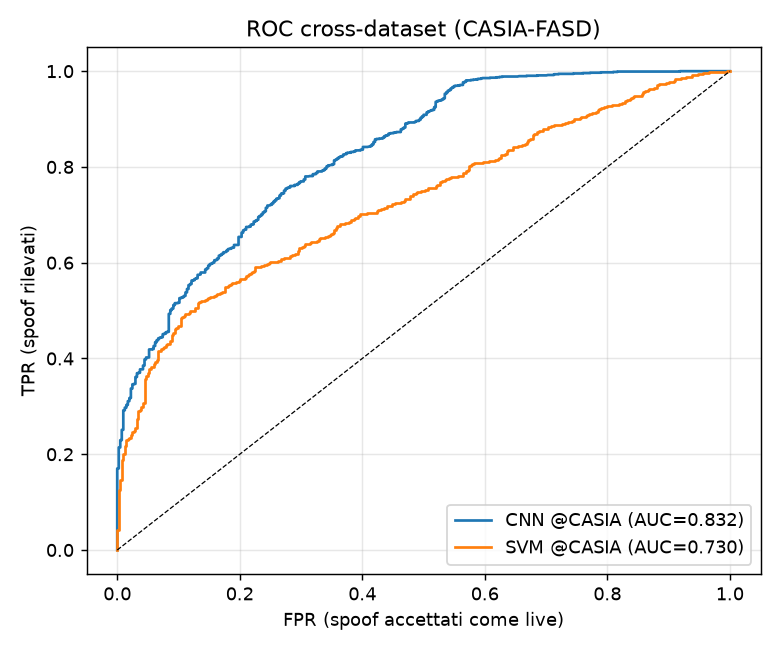
\includegraphics[width=0.58\textwidth]{roc_cross_casia.png}
\caption{ROC sul dataset nuovo (CASIA): entrambi i modelli calano, ma la CNN (AUC 0,83) regge
meglio della baseline (AUC 0,73).}
\end{figure}

\begin{perchebox}
\textbf{Perch\'e fissare la soglia sul val sorgente e non ri-tararla sul target:} nel mondo reale
non conosci in anticipo gli attacchi futuri, quindi devi scegliere la soglia \say{a casa} e
sperare che tenga. Ri-tararla sul dataset nuovo sarebbe \say{barare} (useresti dati che non
avresti). L'\acr{HTER} con soglia fissa misura quindi lo scenario realistico.\\[4pt]
\textbf{Perch\'e questo \`e il pezzo da voto alto:} mostra onest\`a scientifica. Tutti riportano
i numeri belli \say{intra-dataset}; far vedere il \textbf{crollo cross-dataset} (l'HTER della CNN
passa da 7,9\% a 35,4\%) e \textbf{spiegarlo} dimostra che hai capito il vero problema della
biometria: la \textbf{generalizzazione}.
\end{perchebox}

\begin{terminebox}{Cos'\`e il \say{domain gap}}
\say{Dominio} = la distribuzione dei dati (camera, luce, tipo di attacco, etnia\dots). Il
\textbf{domain gap} \`e il calo di prestazioni quando il dominio di test \`e diverso da quello di
training. \`E il limite pratico pi\`u serio dei sistemi anti-spoofing: un modello allenato su un
dataset spesso non regge sugli attacchi \say{nuovi} di un altro. Conclusione del nostro
esperimento: la \textbf{CNN generalizza meglio} della baseline (AUC 0,83 vs 0,73), ma il gap
resta importante.
\end{terminebox}

% =====================================================================
\section{Fase 8 --- Fusione dei due modelli (score-level)}
% =====================================================================
\textbf{Cosa.} Combiniamo gli score di SVM e CNN per vedere se insieme fanno meglio del migliore
da solo. Dato che i due score non sono confrontabili (l'SVM d\`a numeri illimitati, la CNN una
probabilit\`a in $[0,1]$), prima li \textbf{normalizziamo} (min-max, parametri stimati sul val),
poi proviamo varie regole di combinazione (somma, media, prodotto, max, min, somma pesata).

\begin{center}
\small
\begin{tabular}{@{}lrrr@{}}
\toprule
\textbf{Metodo (test)} & \textbf{EER} & \textbf{AUC} & \textbf{ACER} \\
\midrule
CNN (solo)                  & 3,69\% & 0,994  & 3,69\% \\
\textbf{Fusion sum/mean}    & \textbf{3,35\%} & 0,991  & \textbf{3,35\%} \\
Fusion product             & 3,50\% & \textbf{0,9948} & 3,50\% \\
Fusion weighted (w=0,10)   & 5,14\% & 0,987  & 5,14\% \\
\bottomrule
\end{tabular}
\end{center}

\begin{perchebox}
\textbf{Perch\'e fondere:} due modelli che sbagliano su immagini diverse, combinati, si
correggono a vicenda. \`E il \textbf{multi-biometria a livello di score} del corso (Cap.\ 11 del
manuale).\\[4pt]
\textbf{Perch\'e normalizzare prima:} sommare un numero \say{$-3.7$} (SVM) con \say{$0.8$} (CNN)
non ha senso finch\'e non li riporti sulla stessa scala $[0,1]$.\\[4pt]
\textbf{L'insight onesto:} la fusione migliora poco (EER 3,69\% $\rightarrow$ 3,35\%) perch\'e la
CNN \textbf{domina gi\`a} la baseline. E la \say{somma pesata} con peso ottimizzato sul val
\textbf{peggiora} sul test (5,14\%): \`e \textbf{overfitting} del peso sul val. Morale: la regola
semplice (somma a peso uguale) generalizza meglio di quella \say{furba}.
\end{perchebox}

% =====================================================================
\section{Fase 9 --- La demo}
% =====================================================================
\textbf{Cosa.} Una classe \texttt{SpoofDetector} che: trova il volto nel frame (face detector di
OpenCV), lo ritaglia, lo passa alla CNN e restituisce \textbf{LIVE/SPOOF} + lo score. Tre script:
\begin{itemize}
  \item \texttt{single\_image.py}: una foto $\rightarrow$ verdetto + immagine annotata;
  \item \texttt{webcam\_demo.py}: webcam in tempo reale, riquadro \textcolor{green!60!black}{\textbf{verde
        REAL}} / \textcolor{red}{\textbf{rosso SPOOF}};
  \item \texttt{calibrate.py}: cattura qualche tuo frame e fa un mini fine-tuning per adattare il
        modello alla tua webcam/luce.
\end{itemize}

\begin{figure}[h]
\centering
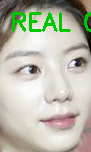
\includegraphics[width=0.42\textwidth]{demo_live.png}
\caption{Esempio di output annotato della demo.}
\end{figure}

\begin{perchebox}
\textbf{Perch\'e una demo:} dimostra che il sistema non \`e solo numeri su un foglio ma
\textbf{funziona davvero} in tempo reale --- l'effetto che colpisce all'orale.\\[4pt]
\textbf{Perch\'e la calibrazione:} il modello \`e allenato su CelebA; la tua webcam \`e un
\say{dominio nuovo} (vedi Fase 7!), quindi pu\`o sbagliare. Catturando qualche tuo frame live/spoof
e ri-allenando 5 epoche, riduci il domain gap \emph{sul tuo setup specifico}. \`E la stessa lezione
della Fase 7 applicata in pratica.
\end{perchebox}

% =====================================================================
\section{Fase 11 --- Riconoscimento e sistema biometrico completo}
% =====================================================================
\textbf{Perch\'e questa fase.} Tutto quello visto finora fa \emph{anti-spoofing} (live vs spoof):
risponde a \say{\`e reale?}, non a \say{chi sei?}. Un sistema biometrico vero fa anche
\textbf{riconoscimento}. Qui aggiungiamo lo stadio mancante e otteniamo la pipeline completa:
\begin{center}
volto $\rightarrow$ \textbf{anti-spoof} (live/spoof) $\rightarrow$ se LIVE $\rightarrow$
\textbf{riconoscimento} (chi sei? / sconosciuto)
\end{center}

\begin{terminebox}{I termini nuovi}
\textbf{Embedding}: un vettore di 512 numeri che rappresenta un volto; foto della stessa persona
$\rightarrow$ vettori vicini, persone diverse $\rightarrow$ vettori lontani.
\textbf{Cosine similarity}: quanto sono \say{allineati} due embedding (1=identici, $\sim$0=diversi).
\textbf{Gallery}: l'archivio degli iscritti (un embedding per soggetto). \textbf{Probe}: la foto
da identificare. \textbf{Verification (1:1)}: \say{sei davvero X?}. \textbf{Identification (1:N)}:
\say{chi sei tra gli N iscritti?}. \textbf{Open-set}: pu\`o anche rispondere \say{nessuno}.
\textbf{rank-1}: \% di probe il cui match corretto \`e il primo della lista. \textbf{CMC}: curva
che mostra il rank-1, rank-2\dots \textbf{MTCNN}: il rilevatore che trova e allinea il volto.
\end{terminebox}

\textbf{Come.} Usiamo \texttt{facenet-pytorch}: \textbf{MTCNN} ritaglia/allinea il volto,
\textbf{InceptionResnetV1} (pre-addestrata su \textbf{VGGFace2}, un grande dataset di volti) lo
trasforma in un embedding da 512 numeri. Confronto tra volti = cosine similarity. La
\textbf{soglia di accettazione} non \`e scelta a occhio: la calibriamo sul benchmark pubblico
\textbf{LFW} (\textit{Labeled Faces in the Wild}).

\begin{perchebox}
\textbf{Perch\'e LFW e non CelebA-Spoof:} il nostro dataset anti-spoofing (cropped) \textbf{non
contiene le identit\`a} dei soggetti, quindi non ci si pu\`o valutare il riconoscimento. LFW \`e
il benchmark standard \emph{con} identit\`a etichettate $\rightarrow$ lo usiamo per misurare il
modulo di recognition e per fissare la soglia. Valutare ogni modulo sul suo benchmark di
riferimento \`e prassi normale.
\end{perchebox}

\textbf{Risultati sul benchmark (LFW).}
\begin{center}\small
\begin{tabular}{@{}lr@{}}
\toprule
\textbf{Compito} & \textbf{Risultato} \\
\midrule
Verification 1:1 (EER) & 3,30\% (AUC 0,974) \\
Identification 1:N (rank-1) & 96,77\% (rank-5 97,80\%) \\
Soglia di accettazione (cosine) & 0,392 \\
\bottomrule
\end{tabular}
\end{center}

\begin{figure}[h]
\centering
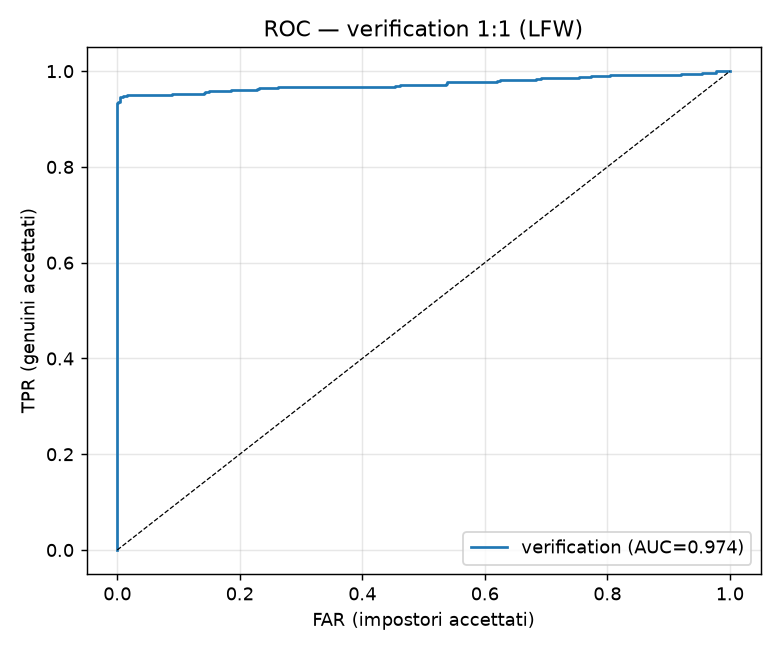
\includegraphics[width=0.46\textwidth]{roc_verification.png}\hfill
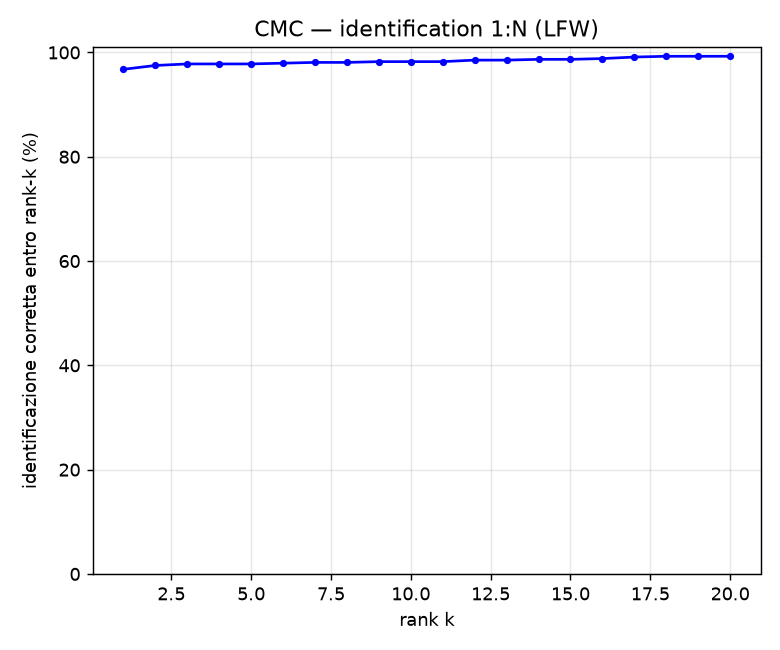
\includegraphics[width=0.46\textwidth]{cmc_identification.png}
\caption{Sinistra: ROC della verification 1:1 su LFW. Destra: curva CMC dell'identification
(rank-1 $\sim$97\%).}
\end{figure}

\textbf{Il test sul tuo scenario (open-set).} Iscriviamo 2 soggetti reali (1 foto a testa) e
proviamo a: (a) riconoscere l'altra foto di ciascuno (\emph{genuini}); (b) rifiutare degli
\emph{impostori} (foto personali + un campione di LFW, garantiti diversi).
\begin{center}\small
\begin{tabular}{@{}lr@{}}
\toprule
\textbf{Esito} & \textbf{Conteggio} \\
\midrule
Genuini identificati correttamente & 2 / 2 \\
Impostori (tuoi) rifiutati & 4 / 4 \\
Impostori (LFW) rifiutati & 50 / 50 \\
\textbf{Falsi accessi} & \textbf{0} \\
\bottomrule
\end{tabular}
\end{center}

\begin{figure}[h]
\centering
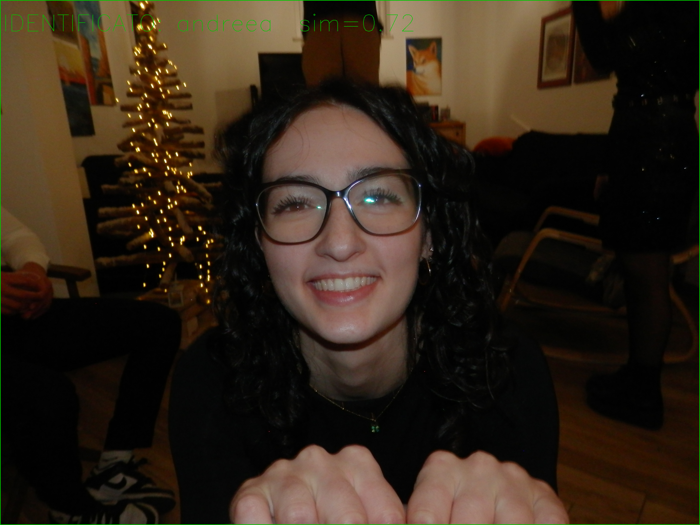
\includegraphics[width=0.40\textwidth]{report_id_genuine.png}\hfill
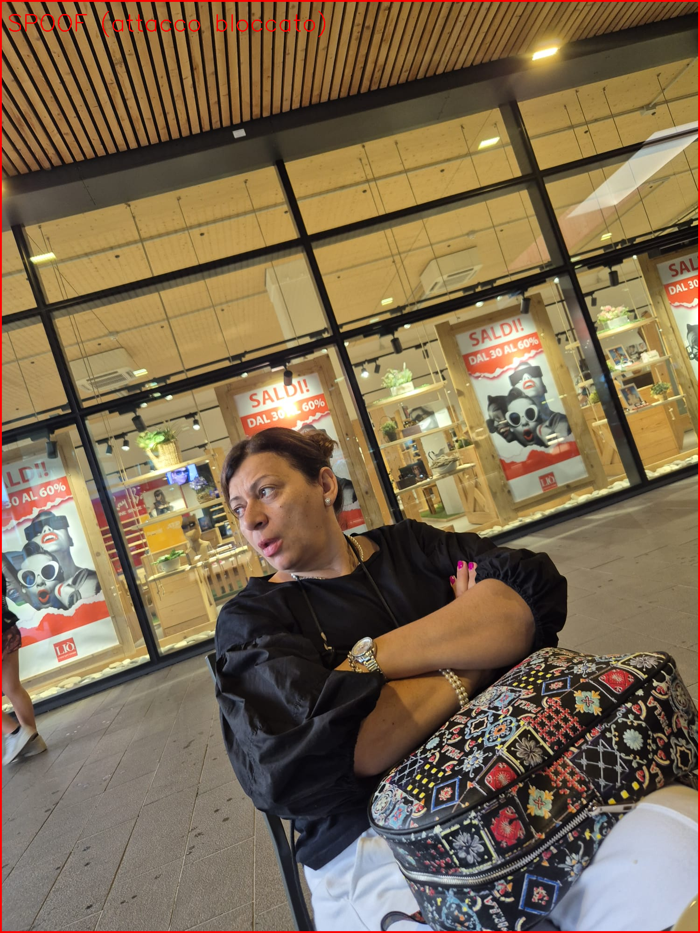
\includegraphics[width=0.40\textwidth]{report_id_impostor.png}
\caption{Sistema completo: a sinistra un genuino (LIVE + IDENTIFICATO), a destra un impostore
(rifiutato).}
\end{figure}

\begin{perchebox}
\textbf{Perch\'e \say{open-set} \`e lo scenario forte:} un sistema da poco \`e \emph{costretto} a
scegliere un nome (closed-set). Qui invece il sistema pu\`o dire \say{SCONOSCIUTO} quando la
similarit\`a col miglior iscritto resta sotto la soglia $\rightarrow$ rifiuta correttamente chi
non \`e in anagrafica. \`E ci\`o che serve nella realt\`a (controllo accessi).
\end{perchebox}

\begin{terminebox}{Nota onesta: l'anti-spoof e il domain gap (ancora)}
Nel test, alcune foto-impostore reali (es. immagini WhatsApp molto compresse) sono state
segnalate come \textbf{SPOOF} pur essendo persone vere. \`E un falso allarme dell'anti-spoof: la
compressione JPEG crea artefatti che il modello, allenato su CelebA-Spoof, scambia per un
attacco --- di nuovo il \textbf{domain gap} della Fase 7. Qui non causa danni (l'impostore viene
comunque rifiutato), ma \`e un limite reale da dichiarare.
\end{terminebox}

% =====================================================================
\section{Risultati in sintesi}
% =====================================================================
\begin{center}
\begin{tabular}{@{}lrr@{}}
\toprule
& \textbf{EER} & \textbf{AUC} \\
\midrule
Baseline SVM (LBP)       & 7,69\% & 0,976 \\
CNN ResNet-18            & 3,69\% & 0,994 \\
Fusione (somma)          & \textbf{3,35\%} & 0,991 \\
\midrule
CNN intra-dataset (HTER) & \multicolumn{2}{c}{7,91\%} \\
CNN cross-dataset (HTER) & \multicolumn{2}{c}{35,36\%} \\
\bottomrule
\end{tabular}
\end{center}

\noindent\textbf{La storia in tre frasi:} (1) il deep learning dimezza l'errore del metodo
classico; (2) la fusione aggiunge un piccolo guadagno; (3) ma tutti i modelli soffrono il
\textbf{domain gap} cross-dataset --- ed \`e l\`a che si gioca la vera ricerca.

% =====================================================================
\section{Come spiegarlo all'orale (cheat-sheet)}
% =====================================================================
\begin{itemize}
  \item \textbf{Cos'\`e:} un classificatore live vs spoof per difendere il riconoscimento
        facciale dagli attacchi di presentazione (foto, schermo, stampa).
  \item \textbf{Due approcci:} feature di texture fatte a mano (LBP) + SVM \emph{vs} CNN che
        impara le feature da sola. La CNN vince (EER 3,7\% vs 7,7\%).
  \item \textbf{Metriche:} EER (punto FAR=FRR), AUC, e le ISO APCER/BPCER/ACER. Pi\`u basso
        l'errore, pi\`u alta l'AUC.
  \item \textbf{Il punto forte:} valutazione \textbf{cross-dataset} (CASIA): le prestazioni
        crollano (HTER 8\% $\rightarrow$ 35\%) $\rightarrow$ il \textbf{domain gap} \`e il vero
        problema della biometria.
  \item \textbf{Fusione:} multi-biometria score-level; normalizzo gli score e li sommo; piccolo
        guadagno; il peso \say{tunato} overfitta $\rightarrow$ meglio la regola semplice.
  \item \textbf{Demo:} funziona in tempo reale con la webcam; la calibrazione applica in pratica
        la lezione del domain gap.
  \item \textbf{Sistema completo (Fase 11):} aggiungo il riconoscimento (embedding facenet +
        cosine), pipeline anti-spoof $\rightarrow$ identificazione \textbf{open-set} (pu\`o dire
        \say{sconosciuto}). Su LFW: verification EER 3,3\%, identification rank-1 97\%. Sul mio
        test: 2/2 genuini identificati, 54/54 impostori rifiutati, 0 falsi accessi.
\end{itemize}

% =====================================================================
\appendix
\section{Appendice A --- Gli script (cosa fa ogni file)}
% =====================================================================
Tutti i percorsi sono relativi alla cartella \texttt{Project - Face Anti-Spoofing/}.
Il codice \say{di libreria} sta in \texttt{src/}; gli eseguibili della demo in \texttt{demo/}.

\renewcommand{\arraystretch}{1.25}
\footnotesize
\begin{xltabular}{\textwidth}{@{}p{3.4cm}cX@{}}
\toprule
\textbf{File} & \textbf{Fase} & \textbf{Cosa fa} \\
\midrule
\endhead
\multicolumn{3}{l}{\textit{src/ --- libreria}}\\[2pt]
\texttt{src/extract.py} & 2 & Estrae i parquet di CelebA-Spoof in PNG su disco + CSV di indice. Risolve l'OOM e scarta le righe corrotte. \\
\texttt{src/data.py} & 2 & \texttt{Dataset} PyTorch che legge i PNG da disco; \texttt{train\_val\_split} (15\% val); \texttt{load\_csv}. Contiene le note anti-leakage. \\
\texttt{src/transforms.py} & 3 & Augmentation per il training e transform per la valutazione; classe \texttt{RandomJPEG}; \texttt{denormalize} per visualizzare. \\
\texttt{src/features\_classic.py} & 4 & Feature color-texture LBP (YCbCr+HSV, 2 scale $\rightarrow$ 168 numeri); estrazione parallela su un DataFrame. \\
\texttt{src/metrics.py} & 4--8 & Tutte le metriche: EER, FAR/FRR, APCER/BPCER/ACER (ISO), HTER, e i plot ROC/DET. Usato da tutte le fasi. \\
\texttt{src/train\_svm.py} & 4 & Baseline: estrae le feature, fit SVM RBF su subset bilanciato, valuta sul test, salva modello + score. \\
\texttt{src/model.py} & 5 & \texttt{build\_model} (backbone timm, testa 2 classi) e \texttt{predict\_scores} (softmax della classe spoof). \\
\texttt{src/train\_cnn.py} & 5 & Training della CNN: AMP, class weights, early stopping su val EER, scheduler cosine. Salva \texttt{cnn\_best.pt} + score test. \\
\texttt{src/evaluate.py} & 6 & Carica gli score salvati, tabella riassuntiva (\texttt{summary.csv}), ROC/DET di confronto; sanity check delle metriche. \\
\texttt{src/cross\_dataset.py} & 7 & Valutazione intra (CelebA) vs cross (CASIA) con soglia fissata sul val sorgente; HTER e gap. \\
\texttt{src/fusion.py} & 8 & Fusione score-level SVM+CNN: normalizzazione min-max (dal val) + regole (sum, mean, product\dots). \\
\texttt{src/infer.py} & 9 & \texttt{SpoofDetector}: carica la CNN, face detection Haar, \texttt{predict}/\texttt{annotate}. Cuore della demo. \\
\texttt{src/recognition.py} & 11 & \texttt{FaceEmbedder}: MTCNN (rileva+allinea) + InceptionResnetV1 $\rightarrow$ embedding 512-d; cosine similarity. \\
\texttt{src/recognition\_eval.py} & 11 & Valutazione su LFW: verification 1:1 (EER) e identification 1:N (rank-1/CMC); calibra la soglia. \\
\texttt{src/biometric\_system.py} & 11 & \texttt{BiometricSystem}: anti-spoof + riconoscimento in cascata; \texttt{enroll} + \texttt{identify} open-set. \\
\texttt{src/openset\_eval.py} & 11 & Test open-set sulla gallery utente: genuini vs impostori (tuoi + LFW); conta i falsi accessi. \\[4pt]
\multicolumn{3}{l}{\textit{demo/ --- eseguibili}}\\[2pt]
\texttt{demo/single\_image.py} & 9 & Una immagine $\rightarrow$ verdetto LIVE/SPOOF + score + immagine annotata salvata. \\
\texttt{demo/webcam\_demo.py} & 9 & Webcam in tempo reale: riquadro verde REAL / rosso SPOOF + FPS. \\
\texttt{demo/calibrate.py} & 9 & Cattura tuoi frame (live/spoof) e fa un mini fine-tuning $\rightarrow$ \texttt{cnn\_calibrated.pt}. \\
\texttt{demo/identify\_image.py} & 11 & Sistema completo su una immagine: live/spoof + identit\`a, immagine annotata. \\
\texttt{demo/identify\_webcam.py} & 11 & Sistema completo in tempo reale: \say{Benvenuto, <nome>} / SPOOF / SCONOSCIUTO. \\
\bottomrule
\end{xltabular}
\normalsize

\subsection*{Ordine di esecuzione (entry-point principali)}
\footnotesize
\begin{enumerate}
  \item \texttt{python src/extract.py} \hfill (Fase 2: parquet $\rightarrow$ PNG + CSV)
  \item \texttt{python src/train\_svm.py} \hfill (Fase 4: baseline)
  \item \texttt{python src/train\_cnn.py} \hfill (Fase 5: CNN)
  \item \texttt{python src/evaluate.py} \hfill (Fase 6: confronto)
  \item \texttt{python src/cross\_dataset.py} \hfill (Fase 7: cross-dataset)
  \item \texttt{python src/fusion.py} \hfill (Fase 8: fusione)
  \item \texttt{python demo/webcam\_demo.py} \hfill (Fase 9: demo)
  \item \texttt{python src/recognition\_eval.py} \hfill (Fase 11: verification/identification su LFW)
  \item \texttt{python src/openset\_eval.py} \hfill (Fase 11: test open-set sulla gallery)
  \item \texttt{python demo/identify\_webcam.py} \hfill (Fase 11: demo sistema completo)
\end{enumerate}
\normalsize
\noindent\textit{Nota:} con Python 3.14 gli script con \texttt{num\_workers>0} vanno lanciati come file
\texttt{.py} reali (il \texttt{DataLoader} usa \texttt{forkserver}).

% =====================================================================
\section{Appendice B --- I dati usati (filepath)}
% =====================================================================
Percorsi relativi a \texttt{Project - Face Anti-Spoofing/}. La cartella \texttt{data/} non \`e
nel repository git (troppo grande, \`e in \texttt{.gitignore}).

\renewcommand{\arraystretch}{1.25}
\footnotesize
\begin{xltabular}{\textwidth}{@{}p{4.2cm}rX@{}}
\toprule
\textbf{Percorso} & \textbf{Dim.} & \textbf{Cos'\`e / a cosa serve} \\
\midrule
\endhead
\multicolumn{3}{l}{\textit{Dati effettivamente usati}}\\[2pt]
\texttt{data/images/} & 12 GB & Le 145.970 immagini PNG (train+test) estratte, organizzate in \texttt{<split>/<live|spoof>/}. Input di training e valutazione. \\
\texttt{data/train.csv} & 79.183 righe & Indice del train: colonne \texttt{filepath,label} (0=live, 1=spoof). \\
\texttt{data/test.csv} & 66.787 righe & Indice del test ufficiale disgiunto (stessa struttura). \\
\texttt{data/casia\_fasd/} & 9,3 MB & CASIA-FASD croppato (1655 volti): il dataset \say{mai visto} del cross-dataset (Fase 7). \\
\texttt{data/casia.csv} & 1.655 righe & Indice di CASIA-FASD (\texttt{filepath,label}). \\
\texttt{data/gallery/<nome>/} & 2 sogg. & Foto dei soggetti da iscrivere (Fase 11): una per l'enrollment, le altre come probe genuini. \\
\texttt{data/impostors/} & 4 foto & Tue foto di persone NON iscritte, per testare il rifiuto (Fase 11). \\
LFW (via \texttt{scikit-learn}) & $\sim$200 MB & Benchmark di face recognition scaricato in automatico (cache \texttt{\textasciitilde/scikit\_learn\_data}); per verification/identification e per la soglia. \\[4pt]
\multicolumn{3}{l}{\textit{Sorgenti scaricate (materiale grezzo)}}\\[2pt]
\texttt{data/celeba\_spoof\_hf/} & 7,0 GB & Parquet del train CelebA-Spoof scaricati da Hugging Face (\texttt{nguyenkhoa/antispoofing}). Input di \texttt{extract.py}. \\
\texttt{data/celeba\_spoof\_test\_hf/} & 4,7 GB & Parquet del test CelebA-Spoof (\texttt{nguyenkhoa/celeba-spoof-...-test}). \\
\texttt{data/casia\_bahareh/} & 6,6 MB & Sorgente CASIA croppato (\texttt{Bahareh0281/CASIA-FASD-Cropped}): zip + \texttt{labels.csv}. \\
\texttt{data/casia\_fasd\_hf/} & 64 KB & Parquet CASIA (sorgente alternativa). \\
\texttt{data/RealDataset (mine)/} & 16 MB & Cartella per tue immagini personali (non usata nelle valutazioni ufficiali). \\
\bottomrule
\end{xltabular}
\normalsize

\subsection*{Output prodotti (cartella \texttt{outputs/})}
\footnotesize
Modelli: \texttt{svm\_baseline.joblib}, \texttt{cnn\_best.pt}.
Score salvati (per la fusione): \texttt{scores\_svm\_test.npz}, \texttt{scores\_cnn\_test.npz}.
Tabelle: \texttt{summary.csv} (Fase 6), \texttt{cross\_dataset.csv} (Fase 7), \texttt{fusion.csv} (Fase 8).
Grafici: \texttt{roc\_*.png}, \texttt{det\_*.png}, \texttt{train\_curve.png}, \texttt{roc\_cross\_casia.png},
\texttt{roc\_fusion.png}, \texttt{aug\_preview.png}, \texttt{crops\_preview.png}, \texttt{demo\_*.png}.
\textbf{Fase 11}: \texttt{recognition\_eval.csv}, \texttt{openset\_results.csv},
\texttt{recog\_threshold.npy}, \texttt{roc\_verification.png}, \texttt{cmc\_identification.png},
\texttt{identify\_*.png}.
\normalsize

\vfill
\begin{center}\small\itshape
Documento di studio personale --- generato dai risultati reali del progetto.
\end{center}

\end{document}
